\chapter{Lattice Boltzmann method}
\vspace{-8mm}
In this chapter, we describe how the equations used in LBM
are derived.
More specifically, we explain
the {\bf Boltzmann transport equation (BTE)}~\cite{mcnamara1988use}, i.e.
the basic equations of the kinetic theory of gases and
how to handle the boundary conditions.

\section{The Boltzmann transport equation (BTE)}
The BTE formulates the time evolution of the 
particle probability density function $f(\xv, \vv, t)$ given
the velocity $\vv$ and the position $\xv$ of particles.
The BTE relaxes the particle distribution to
the Maxwell velocity distribution
function~\cite{huang1963statistical} and the approximation of the relaxation of
$f$ towards $f^{\rm eq}$ is described as follows~\cite{bhatnagar1954model}:
\begin{equation}
  \begin{aligned}
    \od{f(\xv, \vv, t)}{t} &= 
    - \frac{
      f(\xv, \vv, t) - \feq(\vv; \rho(\xv, t), \uv(\xv, t), T(\xv, t))
      }{\tau} \\
    \end{aligned}
    \label{analytical-eq}
  \end{equation}
where $f^{\rm eq}$ is statistical equilibrium,
$T(\xv, t)$ is the temperature at $\xv$
of time step $t$,
$\tau$ is a characteristic time, $\rho(\xv, t)$ is the density
and $\uv(\xv, t)$ is the velocity.
The characteristic time determines how quickly
the fluid converges towards equilibrium.
The higher $\tau$ yields the slower 
convergence towards the equilibrium.
Eq~(\ref{analytical-eq}) is used for the update 
of the particle probability density function.
Furthermore, this particle probability density function
$f(\xv, \vv, t)$ is used for computing
the physical states of the fluid,
such as density and velocity.
The moments updates are performed via~\cite{caroli1984non}:
\begin{equation}
  \begin{aligned}
    \rho(\xv, t) = \int f(\xv, \vv, t) d\vv,~
    \uv(\xv, t) = \frac{1}{\rho(\xv, t)} \int \vv f(\xv, \vv, t)  d\vv 
  \end{aligned}
  \label{analytical-update}
\end{equation}
The underlying equations allow simulating
fluid flow as seen in the latter parts of this paper.

\section{Time-step update of the BTE}
The aforementioned BTE is formulated in the 
continuous domain; therefore,
we need to discretize spatially and 
temporally to make the computation 
feasible by simulations.
In this paper, we focus on discretization
in two-dimensional space.
The discretization for space and time
is performed so that the equality condition of 
the following inequality
(Courant-Friedrichs-Lewy condition) holds~\cite{peyretcomputational, sterling1996stability}:
\begin{equation}
\begin{aligned}
  \cv_i \dt \leq || \Delta \xv_i ||
\end{aligned}
\end{equation}
where $\dt$ is the time step size 
and $\Delta \xv_i$ is the distance between 
the closest grid in the direction
of $\cv_i$ that is defined by:
\begin{equation}
\begin{aligned}
  \cv = \begin{bmatrix}
    0 & 1 & 0 & -1 & 0 & 1 & -1 & -1 & 1 \\
    0 & 0 & 1 & 0 & -1 & 1 & 1 & -1 & -1 \\
  \end{bmatrix}^\top
\end{aligned}
\label{d2q9-velocity}
\end{equation}
Note that this specific discretization in two-dimensional
space with nine directions shown in 
Figure~\ref{fig:d2q9} is called D2Q9.
In this setting, 
we first discretize
the particle probability density function
in the nine directions by subscripting 
as $f_i(\xv, t)$.
Then Eq~(\ref{analytical-update}) becomes the followings:
\begin{equation}
  \begin{aligned}
    \rho(\xv, t) = \sum_i f_i(\xv, t),~
    \uv(\xv, t) = 
    \frac{1}{\rho(\xv, t)} \sum_i \cv_i f_i(\xv) \\
  \end{aligned}
  \label{discretized-momentum}
\end{equation}
Note that we regard the density as
a unit molecular mass in Eq~(\ref{discretized-momentum}).
Additionally, the equilibrium in Eq~(\ref{analytical-eq}) is computed as:
\begin{equation}
\begin{aligned}
  \underbrace{f_i(\xv + \cv_i\dt , t + \dt) - f_i(\xv, t)}_{
    \text{streaming}
  } &= 
  \underbrace{- \omega 
  \biggl[
    f_i(\xv, t) -
    \feq_i(\xv, t)
  \biggl]}_{
    \text{collision}
  }
\end{aligned}
\label{discretized-streaming}
\end{equation}
where $\omega = \dt / \tau$ is the relaxation parameter.
The equilibrium is computed as~\cite{zhao2002non}:
\begin{equation}
\begin{aligned}
  \feq_i(\xv, t) &=
  w_i \rho(\xv, t) \biggl[
    1 + 3 \cv_i \cdot \uv(\xv, t) +
    \frac{9}{2}(\cv_i \cdot \uv(\xv, t))^2
    -\frac{3}{2} || \uv(\xv, t) ||^2
  \biggr] \\
\end{aligned}
\label{discretized-eq}
\end{equation}
where the index $i$ corresponds to Figure~\ref{fig:d2q9}
and $\wv = [\frac{4}{9}, \frac{1}{9}, \frac{1}{9}, \frac{1}{9}, \frac{1}{9}, \frac{1}{36}, \frac{1}{36}, \frac{1}{36}, \frac{1}{36}]$.
In the streaming step, the grid receives 
the particle flow $f_i(\xv + \cv_i \dt, \cdot)$
from its nine adjacent grids.
In the collision step,
we relax the probability density function 
towards the equilibrium $f_i^{\rm eq}$
by considering the effects of the particle collision.

\begin{figure}[h!]
  \begin{center}
   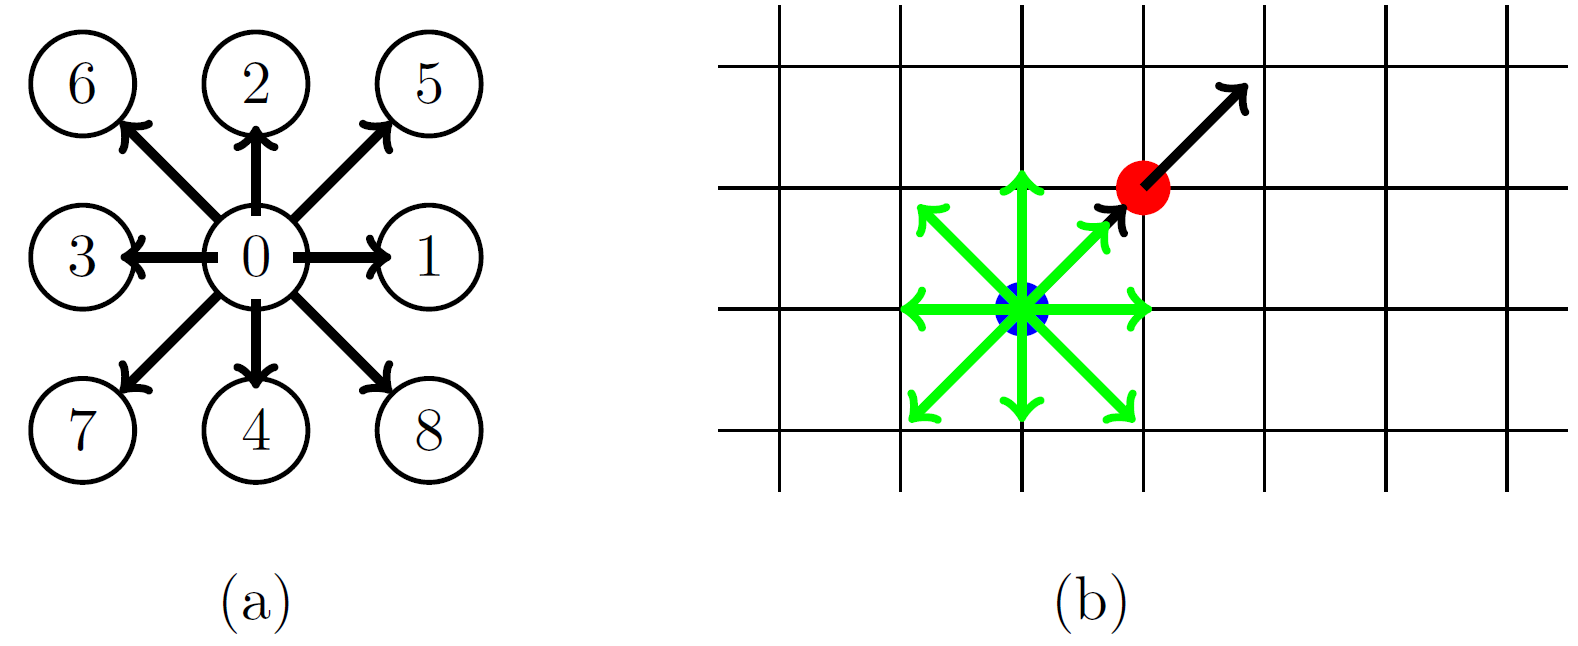
\includegraphics[width=10cm]{logos/Gitter_LBM.png}
   \vspace{-3mm}
   \caption{
      (a) The discretization on the velocity space according to D2Q9.
      (b) The uniform two-dimensional grids for
      the discretization in the physical space.
   }
  \label{fig:d2q9}
  \end{center}
  \vspace{-3mm}
\end{figure}

\section{Boundary handling}\label{boundary-handling-section}
In this section, we briefly discuss how we handle
the particles that bump into boundaries.
Note that the boundary handling is performed
after the streaming step that is discussed in the previous section
and we usually use the direction that is opposite to
the direction $i$ for the bounce-back.
For this reason, we will denote
$f^\star_i$ as the $i$-th direction
particle probability density function
after the streaming step
and $i^\star$ as the direction opposite,
i.e. {\bf reflected direction}, to $i$.
Those directions follow D2Q9 illustrated
in Figure~\ref{fig:d2q9}.
Additionally, there are the following
two ways to
implement the boundary conditions~\cite{liu2014lattice}:
\begin{enumerate}
  \item {\bf Dry nodes}:
  The boundaries are located on the link between nodes
  \item {\bf Wet nodes}:
  The boundaries are located on the lattice nodes
\end{enumerate}
Since the boundary handling will be tedious when
the boundaries are placed on the lattice nodes,
and this is the case for wet nodes,
we use {\bf dry nodes} for the implementation.

\subsection{Bounce-back from objects}\label{boundary-wall-settings}
The most basic boundary condition is 
{\bf rigid wall} or the {\bf bounce-back boundary condition}.
In this condition, we apply the process without
slip condition at the boundary.
The equation at the boundary is computed as~\cite{succi2018lattice}:
\begin{equation}
\begin{aligned}
  f_i(\xv_b, t + \dt) = f_{i^\star}^\star(\xv_b, t)
\end{aligned}
\label{discretized-rigid-wall}
\end{equation}
When the {\bf boundary moves} with the velocity of
$\Uv_w$, the variation in the moments of particles
must be taken into consideration and the equation is
modified as follows~\cite{succi2018lattice}:
\begin{equation}
  \begin{aligned}
    f_i(\xv_b, t + \dt) = f_{i^\star}^\star (\xv_b, t) - 
    2 w_i \rho_w \frac{
      \cv_i \cdot \Uv_w
    }{c_s^2}
  \end{aligned}
  \label{discretized-moving-wall}
\end{equation}
where $c_s$ is the speed of sound and 
$\rho_w$ is the density at the wall.
The computation of $\rho_w$ is usually performed by
either of the followings~\cite{zou1997pressure, khajepor2019study}:
\begin{enumerate}
  \item Take the average density $\bar{\rho}$ of the simulated field
  \item Extrapolate $\rho_w$ using 
  the particle probability density function in the physical domain
\end{enumerate}
For simplicity, we {\bf take the first solution}.

\subsection{Periodic boundary conditions (PBC)}
In this section, we assume that we have
boundaries at $x = 0~(\text{inlet})$ and $X - 1~(\text{outlet})$
where $X$ is the number of the lattice grid in the $x$-axis.
The most basic PBC assumes that
the flow from outlet comes in from inlet as follows~\cite{succi2018lattice}: 
\begin{equation}
\begin{aligned}
  f(0, y, t) = f((X - 1)\dx, y, t)
\end{aligned}
\end{equation}
This condition is implicitly implemented during the streaming operation.
Another PBC handles
the pressure variation $\Delta p$ between inlet and outlet.
Since the density $\rho$ is computed as $\rho = \frac{p}{c_s^2}$
where $p$ is the pressure and $c_s$ is the speed of sound,
the density at the inlet $\rho_{\rm in}$ and
that at the outlet $\rho_{\rm out}$ can be computed
accordingly given the constant pressure $p_{\rm out}$
at the outlet.
Then the prestreaming $f^\star$ at 
the inlet and the outlet are computed as follows~\cite{succi2018lattice}:
\begin{equation}
\begin{aligned}
  f_i^\star(-\dx, y, t) &=
  f_i^{\rm eq}(\rho_{\rm in}, \uv((X - 1)\dx, y, t))
  + (f_i^\star((X - 1)\dx, y, t) - f_i^{\rm eq}((X - 1)\dx, y, t))\\
  f_i^\star(X\dx, y, t) &=
  f_i^{\rm eq}(\rho_{\rm out}, \uv(0, y, t))
  + (f_i^\star(0, y, t) - f_i^{\rm eq}(0, y, t))\\
\end{aligned}
\label{discretized-pbc-pressure}
\end{equation}
where $x = -\dx$ and $x = X\dx$ correspond to $x = (X - 1)\dx$ and $x = 0$
in this setting.
Note that since the pressure PBC computes the prestreaming $f^\star$,
{\bf it must be performed before the streaming operation} unlike the bounce-back.
